\documentclass[landscape]{article}
\usepackage[margin=0.75in]{geometry}
\usepackage{tikz}
\usetikzlibrary{shapes.geometric, arrows, positioning, calc}

% Simplified styling for better fit
\tikzstyle{startstop} = [
    rectangle, 
    rounded corners, 
    minimum width=2.8cm, 
    minimum height=1cm, 
    text centered, 
    draw=black, 
    fill=pink!15, 
    text width=2.6cm, 
    font=\sffamily\small
]

\tikzstyle{process} = [
    rectangle, 
    minimum width=2.8cm, 
    minimum height=1.8cm, 
    text centered, 
    draw=black, 
    fill=orange!15, 
    text width=2.6cm, 
    font=\sffamily\small,
    inner sep=2pt
]

\tikzstyle{decision} = [
    diamond, 
    aspect=2, 
    minimum width=2.8cm, 
    minimum height=1cm, 
    text centered, 
    draw=black, 
    fill=green!15, 
    text width=2cm, 
    font=\sffamily\small,
    inner sep=1pt
]

\tikzstyle{arrow} = [->,>=stealth, thick]
\tikzstyle{note} = [
    rectangle, 
    draw=none, 
    fill=yellow!15, 
    text width=2.2cm, 
    align=left, 
    font=\sffamily\footnotesize
]

\begin{document}
\pagestyle{empty}
\begin{center}
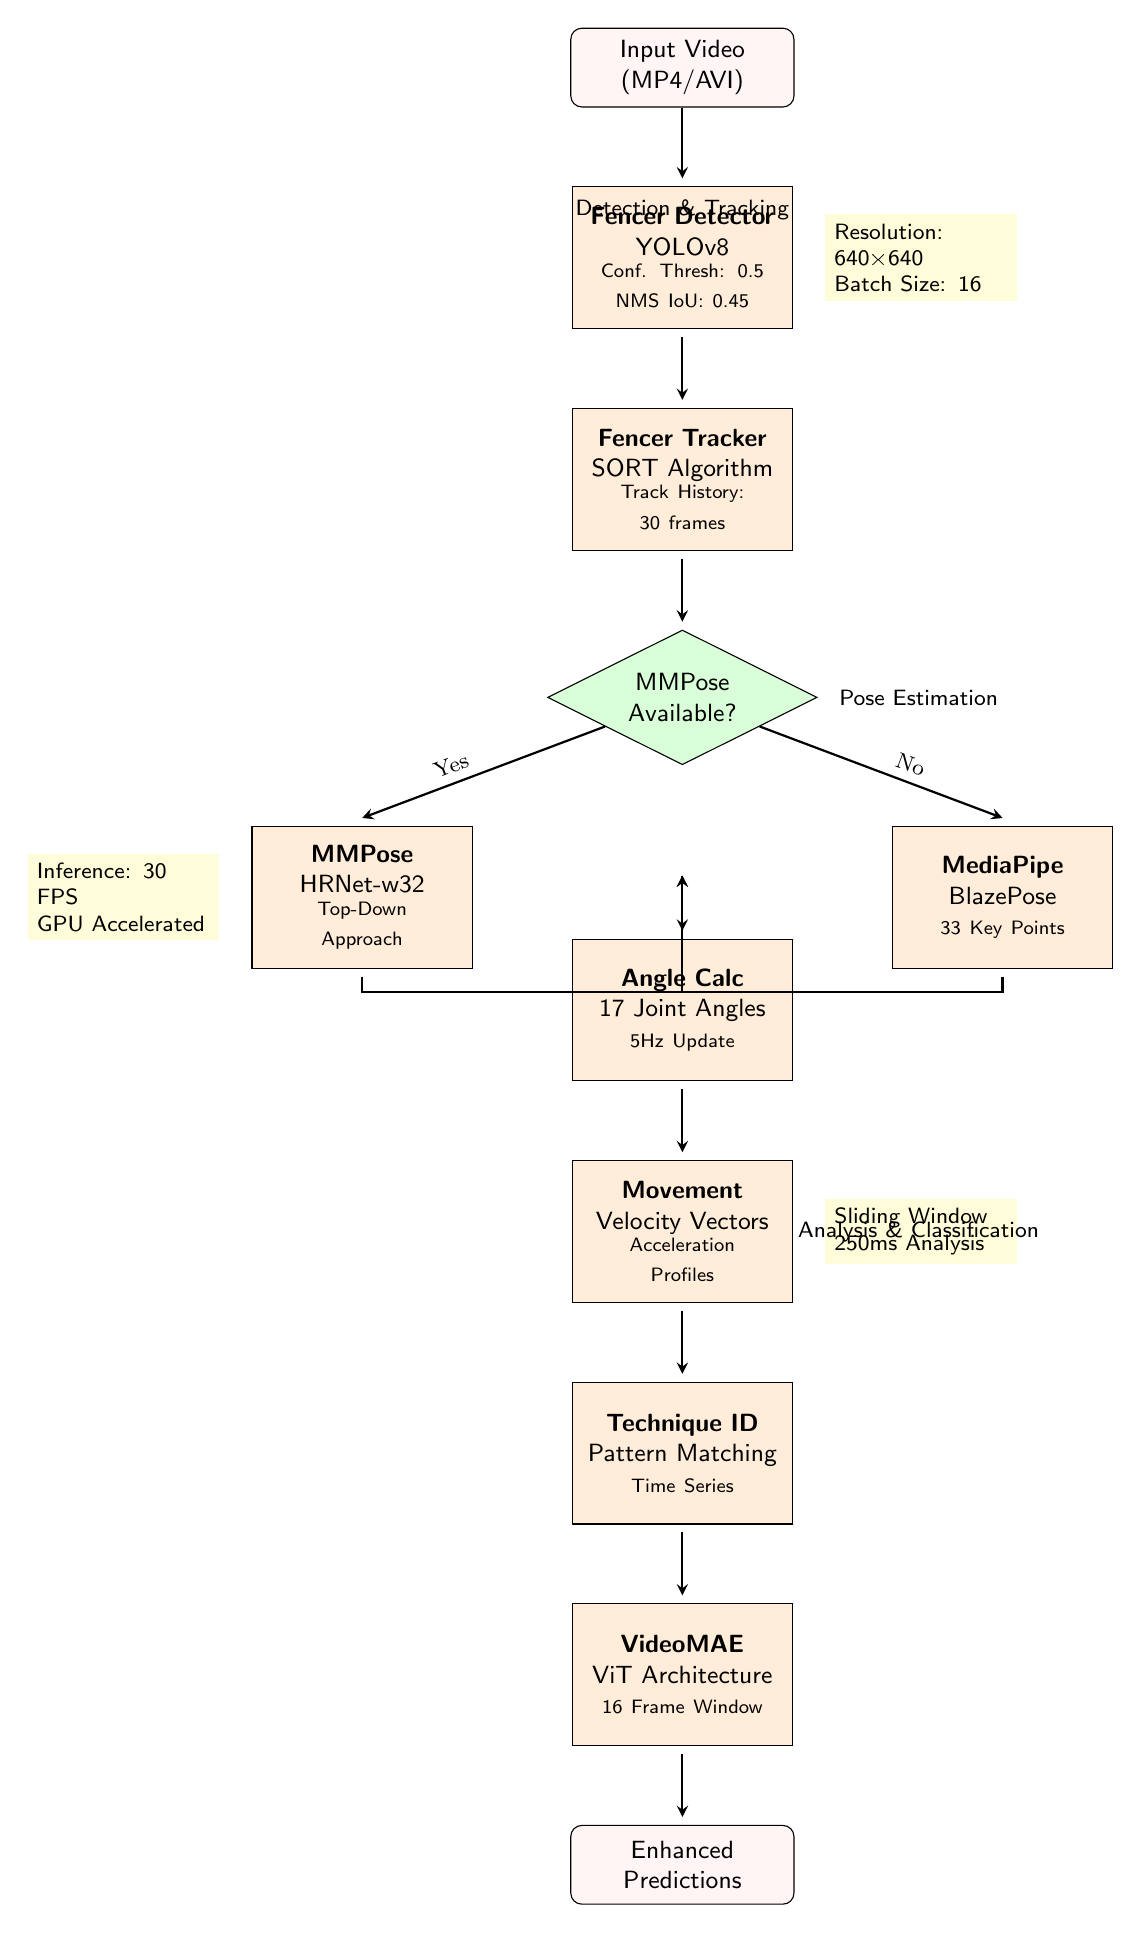
\begin{tikzpicture}[node distance=1.5cm]
    % Input
    \node (input) [startstop] {Input Video\\(MP4/AVI)};
    
    % Detection & Tracking
    \node (detector) [process, below=1cm of input] {
        \textbf{Fencer Detector}\\
        YOLOv8\\
        \scriptsize{Conf. Thresh: 0.5\\NMS IoU: 0.45}
    };
    
    \node (tracker) [process, below=1cm of detector] {
        \textbf{Fencer Tracker}\\
        SORT Algorithm\\
        \scriptsize{Track History:\\30 frames}
    };
    
    % Pose Estimation
    \node (pose_decision) [decision, below=1cm of tracker] {MMPose\\Available?};
    
    \node (mmpose) [process, below left=1.2cm and 1.8cm of pose_decision] {
        \textbf{MMPose}\\
        HRNet-w32\\
        \scriptsize{Top-Down\\Approach}
    };
    
    \node (mediapipe) [process, below right=1.2cm and 1.8cm of pose_decision] {
        \textbf{MediaPipe}\\
        BlazePose\\
        \scriptsize{33 Key Points}
    };
    
    % Analysis
    \node (angle_calc) [process, below=2.2cm of pose_decision] {
        \textbf{Angle Calc}\\
        17 Joint Angles\\
        \scriptsize{5Hz Update}
    };
    
    \node (movement) [process, below=1cm of angle_calc] {
        \textbf{Movement}\\
        Velocity Vectors\\
        \scriptsize{Acceleration\\Profiles}
    };
    
    \node (technique) [process, below=1cm of movement] {
        \textbf{Technique ID}\\
        Pattern Matching\\
        \scriptsize{Time Series}
    };
    
    % VideoMAE
    \node (videomae) [process, below=1cm of technique] {
        \textbf{VideoMAE}\\
        ViT Architecture\\
        \scriptsize{16 Frame Window}
    };
    
    \node (output) [startstop, below=1cm of videomae] {
        Enhanced\\Predictions
    };
    
    % Side notes with better positioning
    \node[note, right=0.4cm of detector] {
        Resolution: 640×640\\
        Batch Size: 16
    };
    
    \node[note, left=0.4cm of mmpose] {
        Inference: 30 FPS\\
        GPU Accelerated
    };
    
    \node[note, right=0.4cm of movement] {
        Sliding Window\\
        250ms Analysis
    };
    
    % Connection points - explicitly create points before and after each node
    \coordinate (input_bottom) at ($(input.south)+(0,-0.1)$);
    \coordinate (detector_top) at ($(detector.north)+(0,0.1)$);
    \coordinate (detector_bottom) at ($(detector.south)+(0,-0.1)$);
    \coordinate (tracker_top) at ($(tracker.north)+(0,0.1)$);
    \coordinate (tracker_bottom) at ($(tracker.south)+(0,-0.1)$);
    \coordinate (pose_decision_top) at ($(pose_decision.north)+(0,0.1)$);
    
    \coordinate (mmpose_top) at ($(mmpose.north)+(0,0.1)$);
    \coordinate (mmpose_bottom) at ($(mmpose.south)+(0,-0.1)$);
    \coordinate (mediapipe_top) at ($(mediapipe.north)+(0,0.1)$);
    \coordinate (mediapipe_bottom) at ($(mediapipe.south)+(0,-0.1)$);
    
    \coordinate (angle_calc_top) at ($(angle_calc.north)+(0,0.1)$);
    \coordinate (angle_calc_bottom) at ($(angle_calc.south)+(0,-0.1)$);
    \coordinate (movement_top) at ($(movement.north)+(0,0.1)$);
    \coordinate (movement_bottom) at ($(movement.south)+(0,-0.1)$);
    \coordinate (technique_top) at ($(technique.north)+(0,0.1)$);
    \coordinate (technique_bottom) at ($(technique.south)+(0,-0.1)$);
    \coordinate (videomae_top) at ($(videomae.north)+(0,0.1)$);
    \coordinate (videomae_bottom) at ($(videomae.south)+(0,-0.1)$);
    \coordinate (output_top) at ($(output.north)+(0,0.1)$);
    
    % Junction point for merging from pose estimators
    \coordinate (junction1) at ($(angle_calc.north)+(0,0.8)$);
    
    % Arrows connecting nodes through connection points
    \draw [arrow] (input.south) -- (detector_top);
    \draw [arrow] (detector_bottom) -- (tracker_top);
    \draw [arrow] (tracker_bottom) -- (pose_decision_top);
    \draw [arrow] (pose_decision) -- node[above left, sloped, font=\footnotesize] {Yes} (mmpose_top);
    \draw [arrow] (pose_decision) -- node[above right, sloped, font=\footnotesize] {No} (mediapipe_top);
    
    % Junction routing with explicit connection points
    \draw [arrow] (mmpose_bottom) -- ++(0,-0.2) -| (junction1);
    \draw [arrow] (mediapipe_bottom) -- ++(0,-0.2) -| (junction1);
    \draw [arrow] (junction1) -- (angle_calc_top);
    
    % Analysis pipeline arrows with connection points
    \draw [arrow] (angle_calc_bottom) -- (movement_top);
    \draw [arrow] (movement_bottom) -- (technique_top);
    \draw [arrow] (technique_bottom) -- (videomae_top);
    \draw [arrow] (videomae_bottom) -- (output_top);
    
    % Section labels
    \node[font=\sffamily\footnotesize] at ($(detector)+(0,0.6)$) {Detection \& Tracking};
    \node[font=\sffamily\footnotesize] at ($(pose_decision)+(3,0)$) {Pose Estimation};
    \node[font=\sffamily\footnotesize] at ($(movement)+(3,0)$) {Analysis \& Classification};
\end{tikzpicture}
\end{center}

\vspace{1cm}

\begin{center}
\textbf{Model Architecture Components}
\end{center}

\begin{itemize}
    \item \textbf{Detection \& Tracking}
    \begin{itemize}
        \item YOLOv8-based fencer detection with real-time optimization
        \item Multi-object tracking using SORT algorithm
        \item Frame-by-frame bounding box refinement
        \item Occlusion handling and ID persistence
    \end{itemize}
    
    \item \textbf{Pose Estimation}
    \begin{itemize}
        \item Primary: MMPose with HRNet-w32 backbone
        \begin{itemize}
            \item Top-down human pose estimation
            \item 17 keypoint detection
            \item GPU-accelerated inference
        \end{itemize}
        \item Fallback: MediaPipe Pose
        \begin{itemize}
            \item CPU-friendly BlazePose model
            \item 33 full-body landmarks
            \item Real-time performance on CPU
        \end{itemize}
    \end{itemize}
    
    \item \textbf{Analysis \& Classification}
    \begin{itemize}
        \item Joint angle calculation
        \begin{itemize}
            \item 17 key joint angles computed
            \item Temporal smoothing with 5Hz update
            \item Anatomical constraints applied
        \end{itemize}
        \item Movement pattern analysis
        \begin{itemize}
            \item Velocity and acceleration profiling
            \item Sliding window analysis (250ms)
            \item Temporal pattern recognition
        \end{itemize}
        \item Technique identification
        \begin{itemize}
            \item Pattern matching against known techniques
            \item Confidence scoring system
            \item Real-time classification
        \end{itemize}
    \end{itemize}
    
    \item \textbf{VideoMAE Integration}
    \begin{itemize}
        \item Pre-trained ViT architecture
        \item 16-frame temporal window
        \item Feature fusion with pose data
        \item Confidence-weighted predictions
    \end{itemize}
\end{itemize}

\end{document} 